\section{January 28, 2021}
\subsection{Inheriting metrics}
A \textbf{Riemannian manifold} is a manifold with a nice, smoothly varying inner product at every point. Given a topological space, how do you come up with an interesting inner product on such space? One way to do this is to sit inside a space that already has one. 
\begin{example}
The inner product of two vectors on the surface of a torus is their inner product in $\R^3$: but how do we actually write this down? We use coordinate charts. Say we have $u,v$ coordinates and a map $(u,v) \to \Sigma(u,v)$. A basis for the domain (in $\R^2$) is just $\partial _u,\partial _v$, so this gives rise to a basis $\partial _u \Sigma=d\Sigma(\partial _u), \partial _v \Sigma=d\Sigma(\partial v)$. These are vectors in $\R^3$. Then 
\[
g_{11}=\partial _u\Sigma \cdot \partial _u\Sigma,\quad g_{12}=g_{21}=\partial _u\Sigma \cdot \partial _v\Sigma,\quad g_{22}=\partial _v\Sigma\cdot \partial _v\Sigma.
\] 
\end{example}
        In general, for a submanifold, take the metric of the big space and restrict it to tangent vectors of the submanifold. When you parametrize surfaces, we need $d\Sigma$ injective (or rank two), or else something else will map to 0, violating the rules of a metric.
        \begin{example}
            Consider the graph $z=f(x,y)$. This gives rise to a simple parametrization, where $\Sigma(u,v)=(u,v,f(u,v))$. Then $\partial _u$ corresponds to $(1,0,\partial _uf)$ and $\partial _v$ corresponds to $(0,1,\partial _vf)$. So \[
                g_{11}=1+(\partial _uf)^2,\quad g_{12}=g_{21}=(\partial _uf)(\partial _vf),\quad g_{22}=1+(\partial _vf)^2.
            \] For the upper hemisphere where $z=\sqrt{1-x^2-y^2} =f(x,y)$, recall that $\partial _u f=-u /\sqrt{1-x^2-y^2} $, $\partial _vf=-v /\sqrt{1-x^2-y^2} $. So \[
            g_{11}=\frac{1-v^2}{1-x^2-y^2},\quad g_{12}=g_{21}=\frac{uv}{\sqrt{1-x^2-y^2} },\quad g_{22}=\frac{1-u^2}{1-x^2-y^2}.
            \] 
        \end{example}
        Work out the metric for the sphere on your own, where $(u,v)\simeq (\theta,\phi) \to (\sin u \cos v, \sin u \sin v, \cos u)$. For a parametrized curve $\gamma (t)$ we only have one component, so $g_{11}=\dot \gamma \cdot\dot \gamma  =\|\dot\gamma \|^2$. So $g=\|\dot\gamma \|^2 dt^2$.

        \subsection{Product spaces}
        Given two manifolds $(M_1,g_1)$ and $(M_2,g_2)$ with coordinates $(x^1,\cdots ,x^n )$, $(y^1,\cdots ,y^m )$, we have the metric $g_1=(g_1)_{ij}dx^i \otimes dx^j $, and the metric $g_2=(g_2)_{k\ell}dy^{k}\otimes dy^{\ell}$. Then we can define the \emph{product manifold} $M_1 \times  M_2$, with coordinates $(x^1,\cdots ,x^n , y^1,\cdots ,y^m)$ Recall from a G\&{}P question that $T_{(p,q)}(M_1\times M_2)=T_pM_1 \times T_q M_2$. So we write a vector $V$ in $T_{(p,q)}(M_1\times M_2)$ in the form $V=(V_1,V_2) $, where $V_1$ is tangent to $M_1$ and $V_2$ is tangent to $M_2$. Then 
        \begin{gather*}
            g=((v_1,v_2),(w_1,w_2))=g(v_1,w_1)+g_2(v_2,w_2) \quad \text{or} \\
            g=g(g_1)_{ij}dx^i \otimes dx^j  + (g_2)_{k\ell}dy^k\otimes dy ^{\ell}.
        \end{gather*}
        The \emph{simplest} example is $\R^2$, where each component is a vector in $\R^1$. Then $g((v_1,v_2),(w_1,w_2))=g_1(v_1,w_1)+g_2(v_2,w_2)=v_1w_1+v_2w_2$, which is exactly how the inner product works in $\R^2$. This generalizes to $\R^{n+m}$, of course.
\begin{example}
    The torus is the product of two circles $\mathbb{T}^2=S^1 _{R_1}\times S^1 _{R_2}$. If the metric on $S^1 _{R_i}$ is given by $R_i^2d\theta^2$, the metric for the torus just $g_1=R_1^2d\theta^2+ R_2^2 d\theta ^2$. 
\end{example}

\subsection{The warped product}
Suppose we have two manifolds $M_1,M_2$ and a function $f \colon M_1 \to \R^+$ (excluding 0!!). Then define $M_1 \times _{f_2}M_2=(M_1 \times  M_2,g)$, where $g$ is \emph{not} the product metric. The metric $g$ at a point $(p,q)$ is given by $g_{(p,q)}=(g_1)_{ij}dx^i  \otimes dx^j +(f(p))^2 (g_2)_{k\ell}dy^k\otimes dy^{\ell}$. This is a \textbf{warped product}. The warped product is indeed a metric, since it's positive definite, given $f(p)$ never maps to zero.

Warped products are familiar: consider surfaces of revolution. If we parametrize $\gamma (t)$ by arc length (so it's unit-speed), then $\gamma (t)=(x(t),y(t))$, a curve in the upper half plane. Then \[
    \Sigma(t,\theta)=(x(t),y(t)\cos (\theta), y(t) \sin \theta).
\] We claim that this surface $\Sigma$ is equal to a product $\gamma \times _f S^1 $, where $f(t)=y$. To see this, note that $\partial _t\Sigma(\dot x,\dot y \cos \theta, \dot y \sin \theta),\ \partial _{\theta}\Sigma=(0,-y \sin \theta,y \cos \theta)$. So $g_{11}=\dot x^2+\dot y^2=1$, $g_{12}=g_{21}=0$, $g_{22}=y^2$. Then our metric is given by $g=dt^2+(y(t))^2d\theta^2$. The reason why $\dot x^2+\dot y^2=1$ is because we used a unit speed parametrization.
\begin{example}
    Concrete example: consider the half circle $\gamma (t)=(\cos t, \sin t)$ for $0<t<\pi$. Then rotating around the $x$-axis gives a sphere minus antipodal poles\footnote{This also omits a line (the IDL?), but we can take care of that by identifying the lines and making the quotient space.}, and $g=dt ^2+\sin ^2(t)d\theta ^2$. This looks very familiar, namely, the metric on this warped product is the exact same as the standard one for the upper half sphere. 

    This demonstrates the idea of the warped product giving an interesting structure. Here, $M_1=(0,\pi)$, $M_2=S^1 $ are both flat, but the warped product gives something round.
\end{example}

\subsection{Quotients by discrete actions}
Consider the quotient space $\R / L\Z$, or the set $\{x\in \R\} / \sim$ where $x \sim (x+nL)$. Does the quotient space inherit a metric? Since $\R/ L\Z$ is a circle, a tangent vector $v_i$ comes from a representative $w_i $ in $\R$, that is $v_i =\pi_*(w_i )$, where $\pi_*$ is projection onto the quotient space. Then define $g(v_1,v_2)=g(w_1,w_2)$. This fails when two vectors upstairs (say $w_i $ and $\widetilde w_i $) have different values under the inner product. For $w_i $ and $\widetilde w_i $ to have the same length, the identification needs to come from a group action by isometries. Here, the group action is ``translate by $L$'', it has no fixed points, and it acts by isometries.

\begin{prop}
    If a group $G$ acts freely on a space $(X,g)$ by isometries, then $X /G$ inherits a metric from $X$. 
\end{prop}
In our example above, $G=\Z$, and the action is $(n,x) \to x+nL$. We are inclined to use the coordinates of $X$ for $X /G$, since locally (pre-identification) $X /G$ looks like $X$. This isn't a new concept, we have done this for years on the circle: we have always used $\theta$ for coordinates by identifying the integers $2\pi n$. When would this fail?
\begin{example}[Non-examples]
    Suppose $X=(\R^+,dx^2)$, and $G=\Z$. Let the action be given by $(n,x)\to 2^n  x$. This is a perfectly nice free group action (by way of our domain). However, $G$ doesn't act by isometries. If we ask what the metric is at 1, this is the same as the metric at 2, 4, $1 /2$, and so on since they're all identified. This group action \emph{stretches} things, so we don't have a well defined notion of length. The quotient is a perfectly good topological space, a circle: it just doesn't have a metric.

    Now suppose $X=\R^2$ and $G=\Z_2$, so the action is rotation by $\pi$. This identifies the lower half of the plane with the upper half, and the positive real axis with the negative real axis. Besides the origin, this is a perfectly good group action acting isometrically and freely. However, the origin is a fixed point. A disk around the origin post quotient becomes a disk $\Z /2$, so this is not a manifold. This is an \emph{orbifold}, a manifold with a singular point. In general, for nonfree group actions, big problems happen in neighborhoods of fixed points.
\end{example}
\begin{example}[Non-non-examples]
    Here we give some actual examples.
    \begin{itemize}
        \item We have already seen $\mathbb{T}^2=\R^2 / \text{lattice} $, where a lattice is $\Z^2$ with two basis vectors. In general, we can form $\mathbb{T}^n =\R^n / \text{lattice}  $.
        \item Another important example is $\R \mathrm P^n=S^n /\pm 1$.
        \item The \textbf{lens spaces} $L(p,q)$ are formed by taking $S^3 \subseteq \C^2 / \sim$, where $(z_0,z_1)\sim (\lambda z_0,\lambda^q z_1)$ and $\lambda =e^{2\pi i /p}$. The group here is $\Z_p$, and the identification is the group action, acting by isometries with no fixed points. Note that we want $p,q$ to be relatively prime. Also note that $L(2,1)$, since $e^{2\pi i/ 2}=-1$. These lens spaces look locally like $S^3$, but globally have some interesting topological properties: namely $\pi_1(L(p,q))=\Z_p$.
        \item We will also eventually see some Riemann surfaces, given by $\H^2 /G$. Hyperbolic space has constant negative curvature, so you can realize a structure of Riemann surfaces with genus greather than 1, and give them all metrics of constant negative curvature. This is the same thing as talking about the \emph{canonical} space of constant curvature $\H$, and modding it by a certain group action.
    \end{itemize}
\end{example}

\subsection{The complex projective plane}
We can also quotient by continuous groups. Consider the complex projective plane $\C\mathrm P^1$, defined by \[
    \C \mathrm P^1 := \big\{(z_1,z_2)\in \C^2\setminus \{0\} \big\} /\sim,\quad (z_1,z_2)\sim (\lambda z_1,\lambda z_2),\ \lambda \in \C\setminus \{0\} =\C^*.
\] Multiplication by a scalar $\lambda$ (say $3+i$) is \emph{not} an isometry, since it scales lengths by $\sqrt{10} $. So the way we've written it as of now doesn't fit into our framework. However, we can break up $\C^*$ into $\R^+\times U(1) $\footnote{Recall that $U(1)$ denotes the unit complex numbers.}, an element of the unit circle times a length. So we can rewrite the definition as \[
\C\mathrm P^1 :=\big\{(z_1,z_2)\in \C^2\mid (z_1)^2+(z_2)^2=1\big\} / \sim,\quad (z_1,z_2)\sim (e^{i\theta}z_1,e^{i\theta}z_2) .
\] Behold, \emph{this} is an isometry. For now we restrict our discussion to lengths of vectors, since if you know what the length of a vector is, you know what the inner product is. This is because $\langle v,w \rangle =(\langle v+w,v-w \rangle -\langle v-w,v-w \rangle )/4$ which is the sum of lengths squared over four. (This is called the \emph{polarization identity}.) Consider $S^3 \subseteq \C^2 $ projecting onto $\C\mathrm P^1$ (topologically a sphere) by $\pi$, then a point $p \in \C \mathrm P^1$ corresponds to a circle in $S^3$. Consider a point $q$ in this circle in $S^3$ corresponding to $p$. 

\begin{figure}[H]
\centering
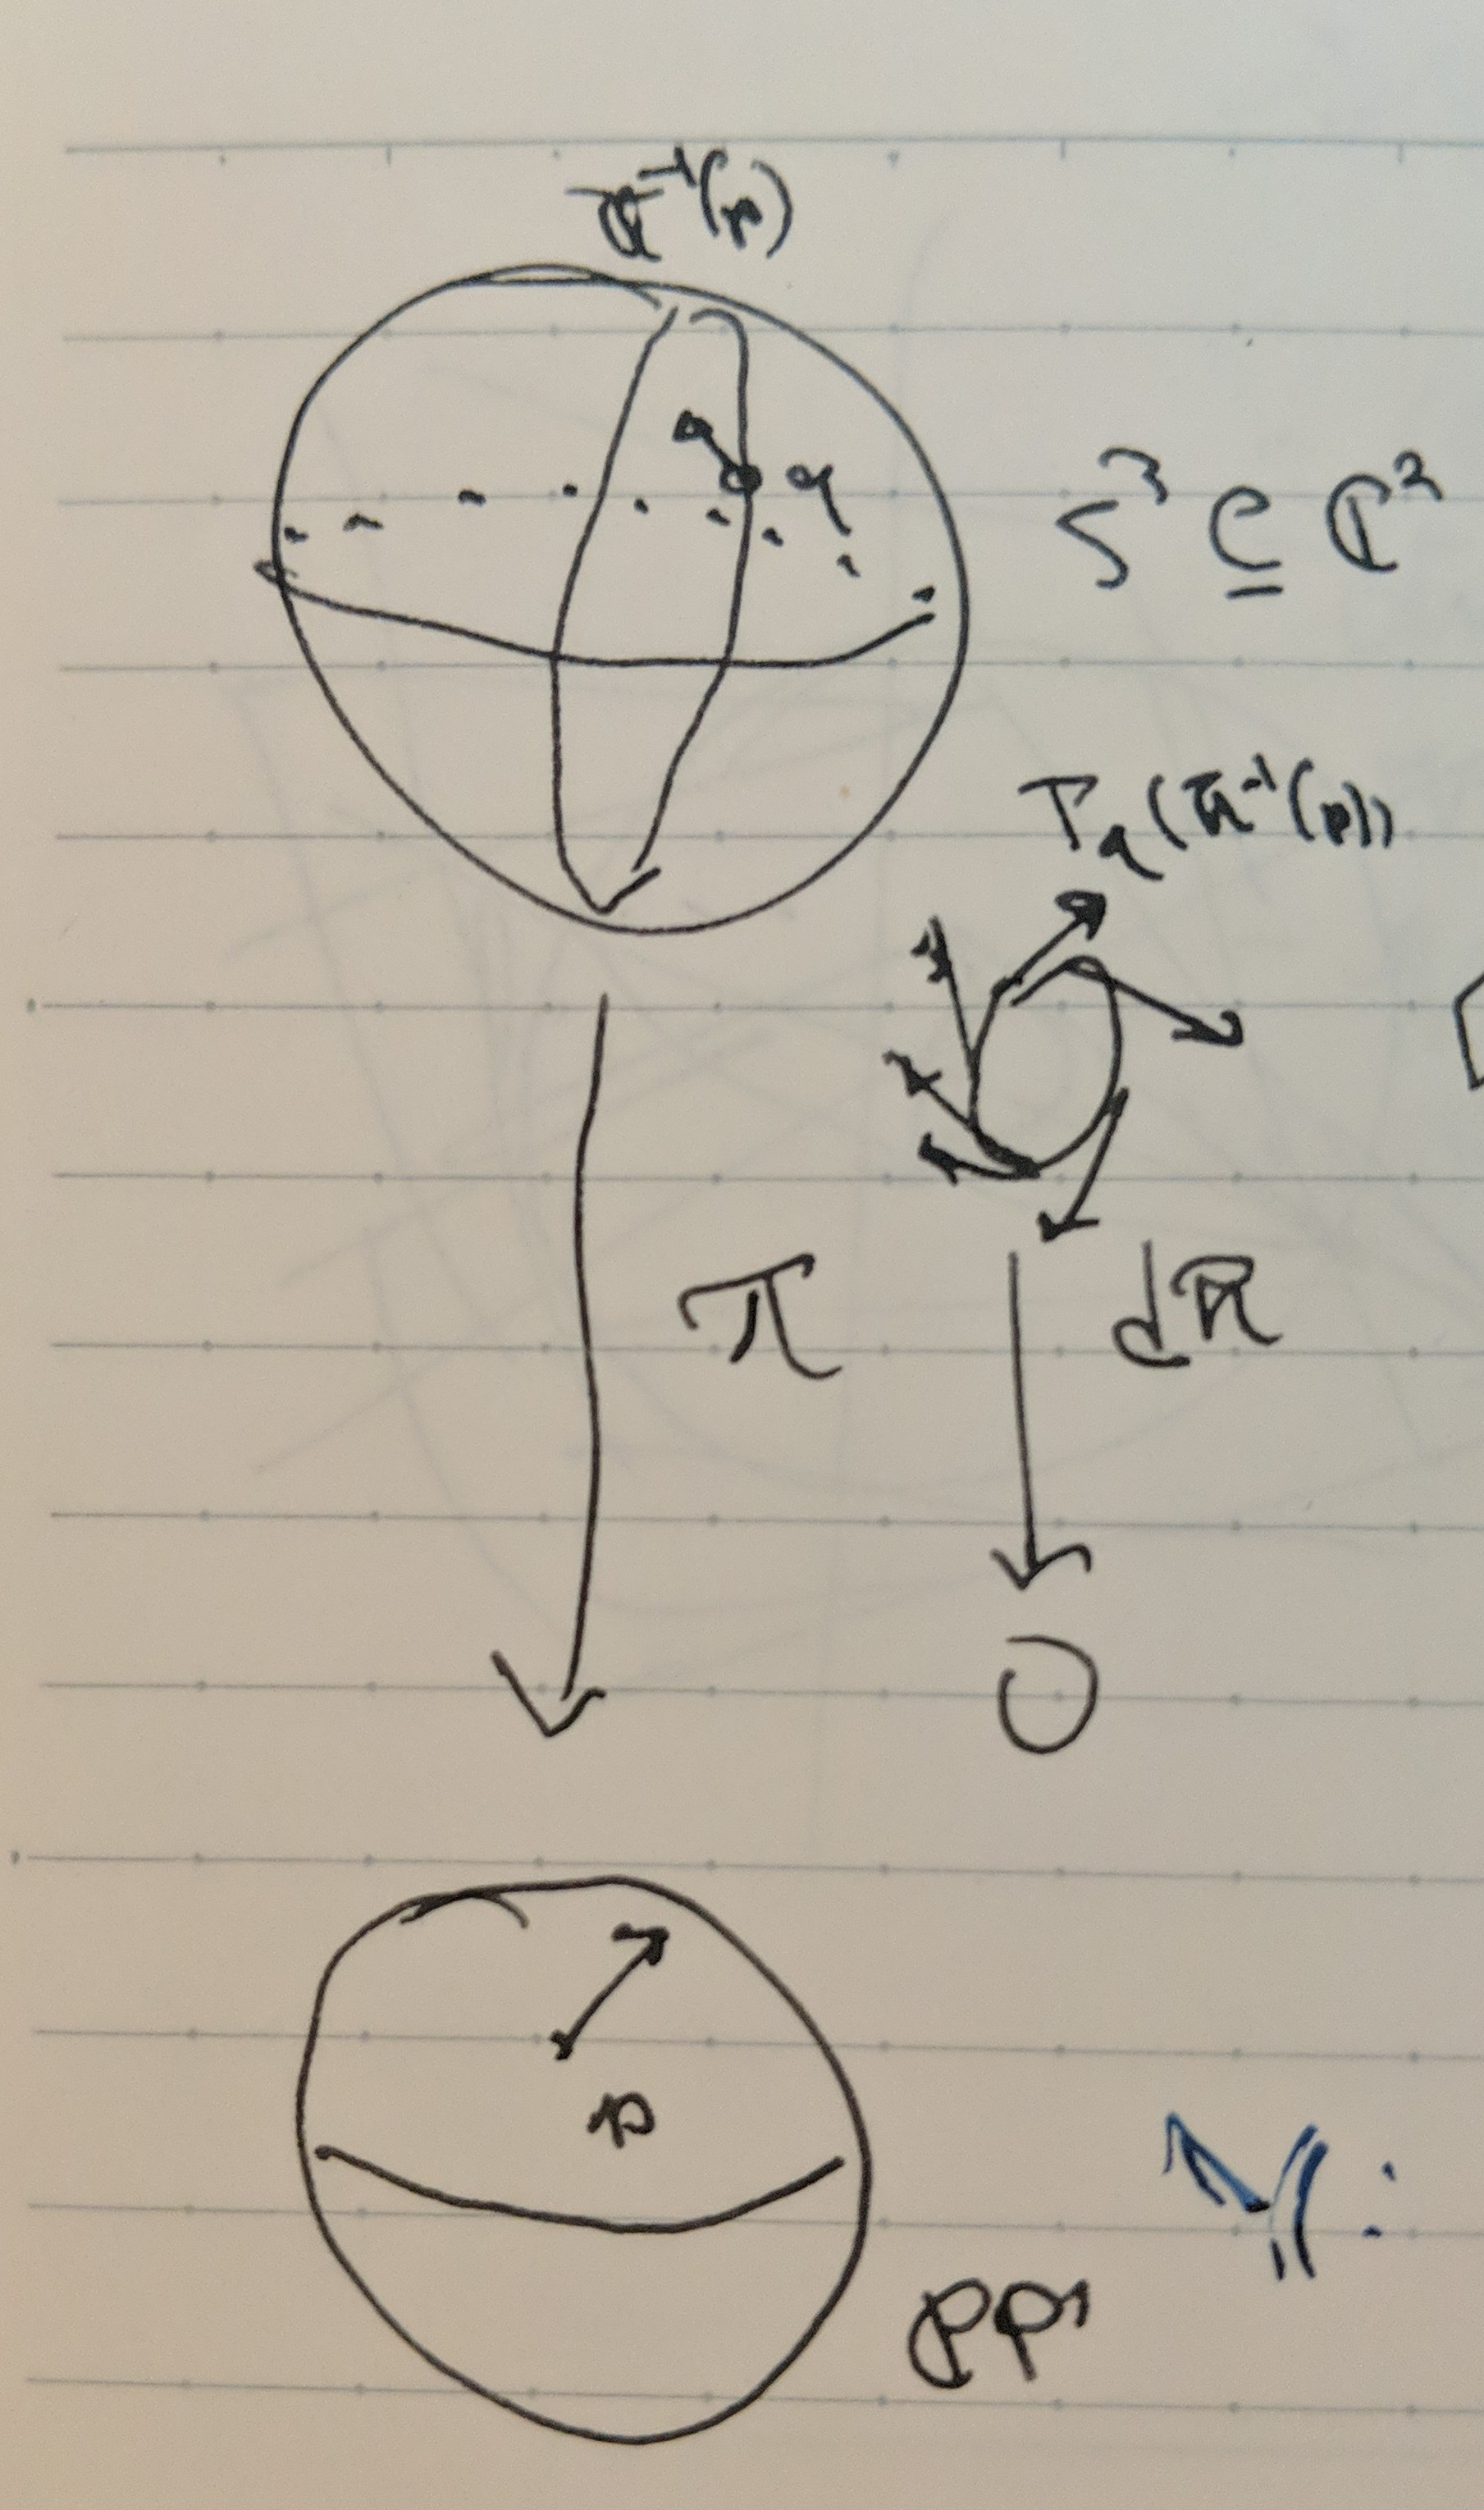
\includegraphics[width=0.3\linewidth]{figures/rgeo_lec4.jpg}
\end{figure}

However, $d\pi$ is \emph{not} injective, since it maps any vector tangent to the sphere to zero. We can write $T_q S^3$ as $T_q (\pi ^{-1}(p))+T_q(\pi ^{-1}(p))^{\perp}$, so $d\pi \colon T_q(\pi ^{-1}(p)) \to 0$. But $d\pi \colon T_q(\pi ^{-1}(p))^{\perp} \to T_p \C \mathrm P^1$ is an isomorphism by the rank nullity theorem, since $T_q(\pi ^{-1}(p))=\ker d\pi$. Let us name this map $\alpha $. Then $\langle v,w \rangle =g(\alpha ^{-1}(v),\alpha ^{-1}(w))$. We say the vectors $T_q(\pi ^{-1}(p))$ are \textbf{vertical}, or they live in the fiber above a point. A vector that lives in $T_q(\pi ^{-1}(p))^{\perp}$ is \textbf{horizontal}, since it's orthogonal to a vertical vector. So the idea is to lift vectors in the base space uniquely to \emph{horizontal} vectors, since they don't generally have a unique vertical left (since $d\pi$ fails to be injective). What ingredients did we need to make this work?
\begin{enumerate}[label=(\arabic*)]
    \item The group acts by isometries. (We need two distances in the total space to be the same.)
    \item The group needs to act freely.
\end{enumerate}
This map $\pi$ from $S^3\to S^2$ is called the \textbf{Hopf fibration}. This map has some nice properties, that is, the preimage of two points will always be linked circles (if you think of $S^3$ as the one-point compactification of $\R^3$). For $\C\mathrm P^n $, we consider it as the quotient $S^{2n+1} / S^1 $, or $S^{2n+1}=\{(z_0,\cdots ,z_n )\mid |z_0|^2+\cdots +|z_n |^2=1\} / S^1 $, where $(z_0,\cdots ,z_n )\sim (e^{i\theta}z_1,\cdots ,e^{i\theta}z_n )$. What does the metric on $\C\mathrm P^1$ look like? This is the \textbf{Fubini-Study metric} {\color{red}todo:read about this in the book} 
